\documentclass[usenames,dvipsnames,serif,14pt]{beamer}%
\usetheme{Copenhagen}%
\usepackage[utf8]{inputenc}%
\usepackage[english]{babel}%
\usepackage{amsmath}%
\usepackage{amsfonts}%
\usepackage{amssymb}%

% for image
\usepackage{graphicx}%
% font and style package
\usepackage{mathpazo}%
% url handling
\usepackage{url}%
% code hilighting
\usepackage{minted}%
% load more color name (in conjuction with dvipsname)
\usepackage{xcolor}
% for algorithm
\usepackage[french, onelanguage]{algorithm2e}
\usepackage{algorithmic}
% for tree
\usepackage{tikz}

%for floaw chart
\usetikzlibrary{arrows.meta}
\tikzset{%
  >={Latex[width=2mm,length=2mm]},
  % Specifications for style of nodes:
            base/.style = {rectangle, rounded corners, draw=black,
                           minimum width=4cm, minimum height=1cm,
                           text centered, font=\sffamily},
  mainFile/.style = {base, fill=blue!30},
       subFile/.style = {base, fill=red!30},
    module/.style = {base, fill=green!30},
        % process/.style = {base, minimum width=2.5cm, fill=orange!15,font=\ttfamily},
}

\usepackage{ragged2e}



\RestyleAlgo{boxruled}
\SetAlCapHSkip{0.5em}
\IncMargin{1em}

\author{Nicolas Bailluet, Rémi Piau}
\title{Projet 0: Tours de Hanoï et Pavage de Penrose}

\usecolortheme[named=Mahogany]{structure}
%\setbeamercovered{transparent}
%\setbeamertemplate{navigation symbols}{}
%\logo{}
\institute{L3, ENS Rennes}
\date{Septembre 2018}

% Custom commands
\newcommand{\ZZ}{\mathbb{Z}}
\newcommand{\NN}{\mathbb{N}}
\newcommand{\ddp}{\displaystyle}
%\subject{}

% Fine tuning
%\setlength{\parskip}{0.5\baselineskip}%
%%%
%%%
% SET FRAME TO [fragile] whenever you have to use minted !!!

\begin{document}
\beamertemplatenavigationsymbolsempty

\begin{frame}
\titlepage
\end{frame}

\section{Pavage de Penrose}
\begin{frame}[fragile]%{•}
\frametitle{Une implémentation modulaire}
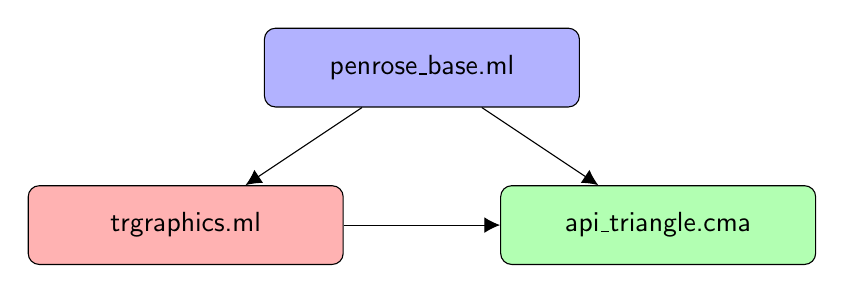
\begin{tikzpicture}[node distance=1.5cm,
    every node/.style={fill=white, font=\sffamily}, align=center]
  % Specification of nodes (position, etc.)
  \node (penrosebase) at (0,0)           [mainFile]          {penrose\_base.ml};
  \node (trgraphics) at (-3,-2)     [subFile]        {trgraphics.ml};
  \node (apitriangle) at (3, -2)     [module] {api\_triangle.cma};   
  % Specification of lines between nodes specified above
  % with aditional nodes for description 
  \draw[->]             (penrosebase) -- (apitriangle);
  \draw[->]     (penrosebase) -- (trgraphics);
  \draw[->]      (trgraphics) -- (apitriangle);
\end{tikzpicture}
\end{frame}

\begin{frame}[fragile]%{•}
\frametitle{Une API pour les triangles}
\begin{minted}{ocaml}
type point
type coord = int * int
type triangle
val ( -- ) : point -> point -> point
val ( // ) : point -> float -> point
val norm : point -> float
val new_point : float -> float -> point
val is_acute : triangle -> bool

\end{minted}
\end{frame}

\begin{frame}[fragile]%{•}
\frametitle{Le pavage un algorithme recursif}
\scalebox{0.99}{  
  \begin{algorithm}[H]
  \SetKwInOut{Input}{Entrées}
  \caption{Penrose($n$, $t$)}
  \Input{$n$ : nombre de générations, \newline
  $t$ : triangle initial}
  \eIf{$n = 0$}{ dessiner $t$}
  { Découper $t$ et appliquer Penrose($n-1$,$t_i$) pour chaque sous triangle $t_i$.
   }
  \end{algorithm}
  }
\end{frame}



\begin{frame}[fragile]%{•}
\frametitle{Amélioration: déplacement au clavier}
	\begin{center}
    		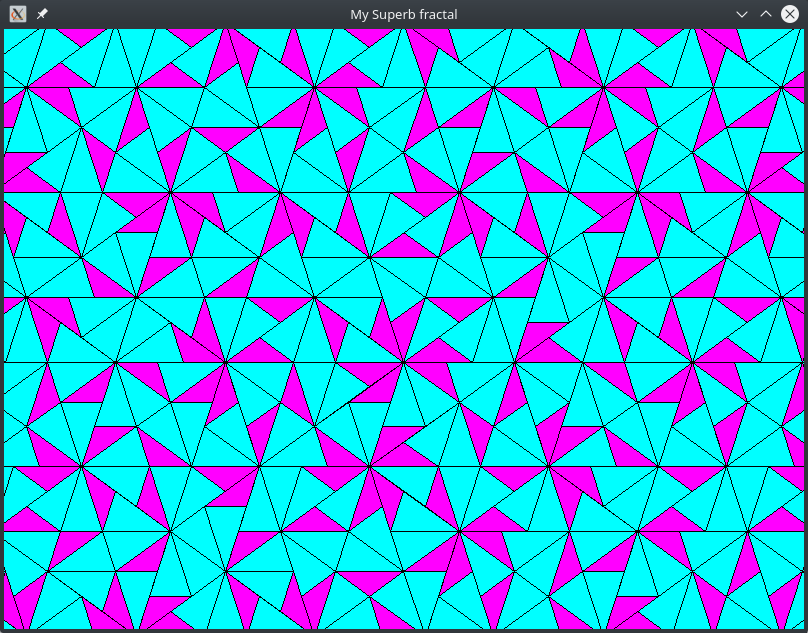
\includegraphics[scale=0.3]{penrose_anime.png}
    \end{center}
\end{frame}
\section{Tours de Hanoï}

\begin{frame}{Algorithme récursif optimal}
  \begin{algorithm}[H]
  \SetKwInOut{Input}{Entrées}
  \caption{Hanoi($n$, $s$, $i$, $d$)}
  \Input{$n$ : nombre de disques, \newline
  $s$ : piquet de départ, \newline
  $i$ : piquet intermédiaire, \newline
  $d$ : piquet d'arrivée}
  \If{$n > 1$}{ Hanoi($n-1$, $s$, $d$, $i$)\\
                Déplacer un disque de $s$ vers $d$\\
                Hanoi($n-1$, $i$, $s$, $d$)}
  \end{algorithm}
\end{frame}

\begin{frame}{Complexité}
  \centering
  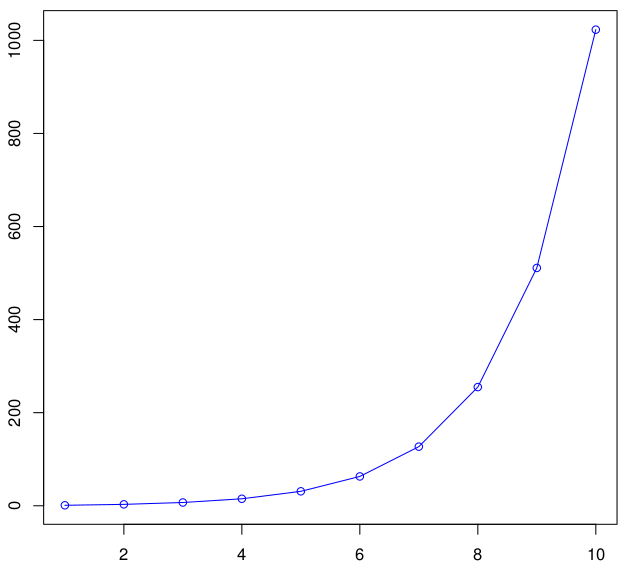
\includegraphics[scale=0.2]{R_curve.png}
  \begin{block}{Calcul}
    $C(n) =
    \begin{cases}
      1 & \mbox{si $n$ = 1}\\
      2C(n)+1 & \mbox{sinon}
    \end{cases}
    $
    $\Leftrightarrow \boxed{C(n) = 2^{n}-1}$
  \end{block}
\end{frame}


\begin{frame}{Représentation sous forme d'arbre}
  \begin{block}{Construction de l'arbre}
  \begin{center}
  \scalebox{0.5}{
  \begin{tikzpicture}[auto,
    every node/.style={circle,minimum size=3.5em},
    level/.style = {sibling distance=6em}]
    \node[draw]{$n$}
    child {node[draw](a){$n-1$}
      child {node{$\vdots$}
        child {node[draw]{$1$}}
        child {node{$\cdots$}}
      }
      child {node{$\vdots$}}
    }
    child {node(b)[draw]{$n-1$}
      child {node{$\vdots$}}
      child {node{$\vdots$}
        child {node{$\cdots$}}
        child {node[draw]{$1$}}
      }
    };
  \end{tikzpicture}}
  \end{center}
  \begin{itemize}
    \justifying
    \item Disques indicés (taille croissante) de 1 à $n$.
    \item Arbre complet de hauteur $n$.
  \end{itemize}
  \end{block}
\end{frame}

\begin{frame}{Parcours infixe}
  \begin{block}{Ordre de déplacement des disques}
    \begin{itemize}
    \item
    $n=4$:
      \begin{center}
        $(1, 2, 1, 3, 1, 2, 1, 4, 1, 2, 1, 3, 1, 2, 1)$
      \end{center}
    \item
    $n=3$:
      \begin{center}
        $(1, 2, 1, 3, 1, 2, 1)$
      \end{center}
    \end{itemize}
  \end{block}
  \begin{block}{Résultat}
    \justifying
    L'indice du disque joué au tour d'ordre $k$
    correspond à l'indice du premier bit nul dans l'écriture binaire de $k$.
  \end{block}
\end{frame}

\begin{frame}{Algorithme itératif optimal}
  \begin{center}
  \scalebox{0.80}{
  \begin{algorithm}[H]
  \SetKwInOut{Input}{Entrées}
  \caption{Hanoi($n$, $s$, $i$, $d$)}
  \While{hauteur($d$) $< n-1$}
  {
    \eIf{$n$ est pair}
      {Déplacer le plus petit disque d'un piquet vers la droite}
      {Déplacer le plus petit disque d'un piquet vers la gauche}
    Effectuer le seul mouvement qui ne déplace pas le plus petit disque
  }
  Déplacer le plus petit disque vers $d$
  \end{algorithm}}
  \end{center}
\end{frame}

\begin{frame}[fragile]{Implémentation}
  \begin{block}{Type abstrait \textit{Rod}}
    \begin{minted}{ocaml}
    type rod
    val push : rod -> int -> unit
    val pop : rod -> int
    val is_empty : rod -> bool
    val top : rod -> int
    val init_rod : int -> string -> rod
    val move : rod -> rod -> unit
    val get_size : rod -> int
    val get_name : rod -> string
    \end{minted}
  \end{block}
\end{frame}

\begin{frame}{Implémentation}
  \begin{block}{Animation de la résolution}
    \begin{center}
    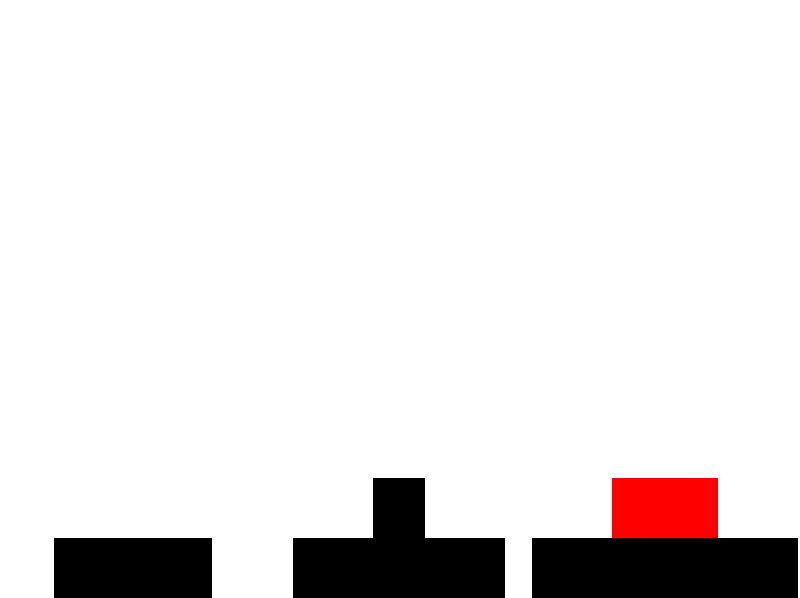
\includegraphics[scale=0.2]{anim_hanoi.png}
    \end{center}
  \end{block}
\end{frame}

\section{Conclusion}
\begin{frame}
\frametitle{Pistes d'amélioration}
  \begin{block}{Penrose}
  	\begin{itemize}
  	\item Rotation dans l'animation.
  	\item Pouvoir revenir dans les générations.
  	\item Implémenter d'autres pavages (plus jolis).
  	\end{itemize}
  \end{block}
  \begin{block}{Hanoi}
  	\begin{itemize}
  	\item Plus de piquets (Frame-Stewart).
  	\item Résolution à partir d'un état quelconque.
  	\item Meilleure animation (plus jolie).
  	\end{itemize}
  \end{block}
\end{frame}

\end{document}
